\begin{frame}[c]
  \myframetitle{Aufgabe 2}{Suche mittels Page-Rank}
\begin{itemize}
  \fatitem{Der Page-Rank ist die Wahrscheinlichkeit eines Websiten-Besuchs}
  \item Das Ranking der Websites kann offline erfolgen
  \item Für die Übung wurde das Iterative Pagerank-Verfahren implementiert
  \item Der Algorithmus konvergiert nach 30 Iterationen auf dem Beispielgraph
\end{itemize}
\end{frame}

\begin{frame}[c]
\myframetitle{Page-Rank}{Verteilung des Page-Ranks}
%\usepackage{graphics} is needed for \includegraphics
\begin{figure}[htp]
\begin{center}
  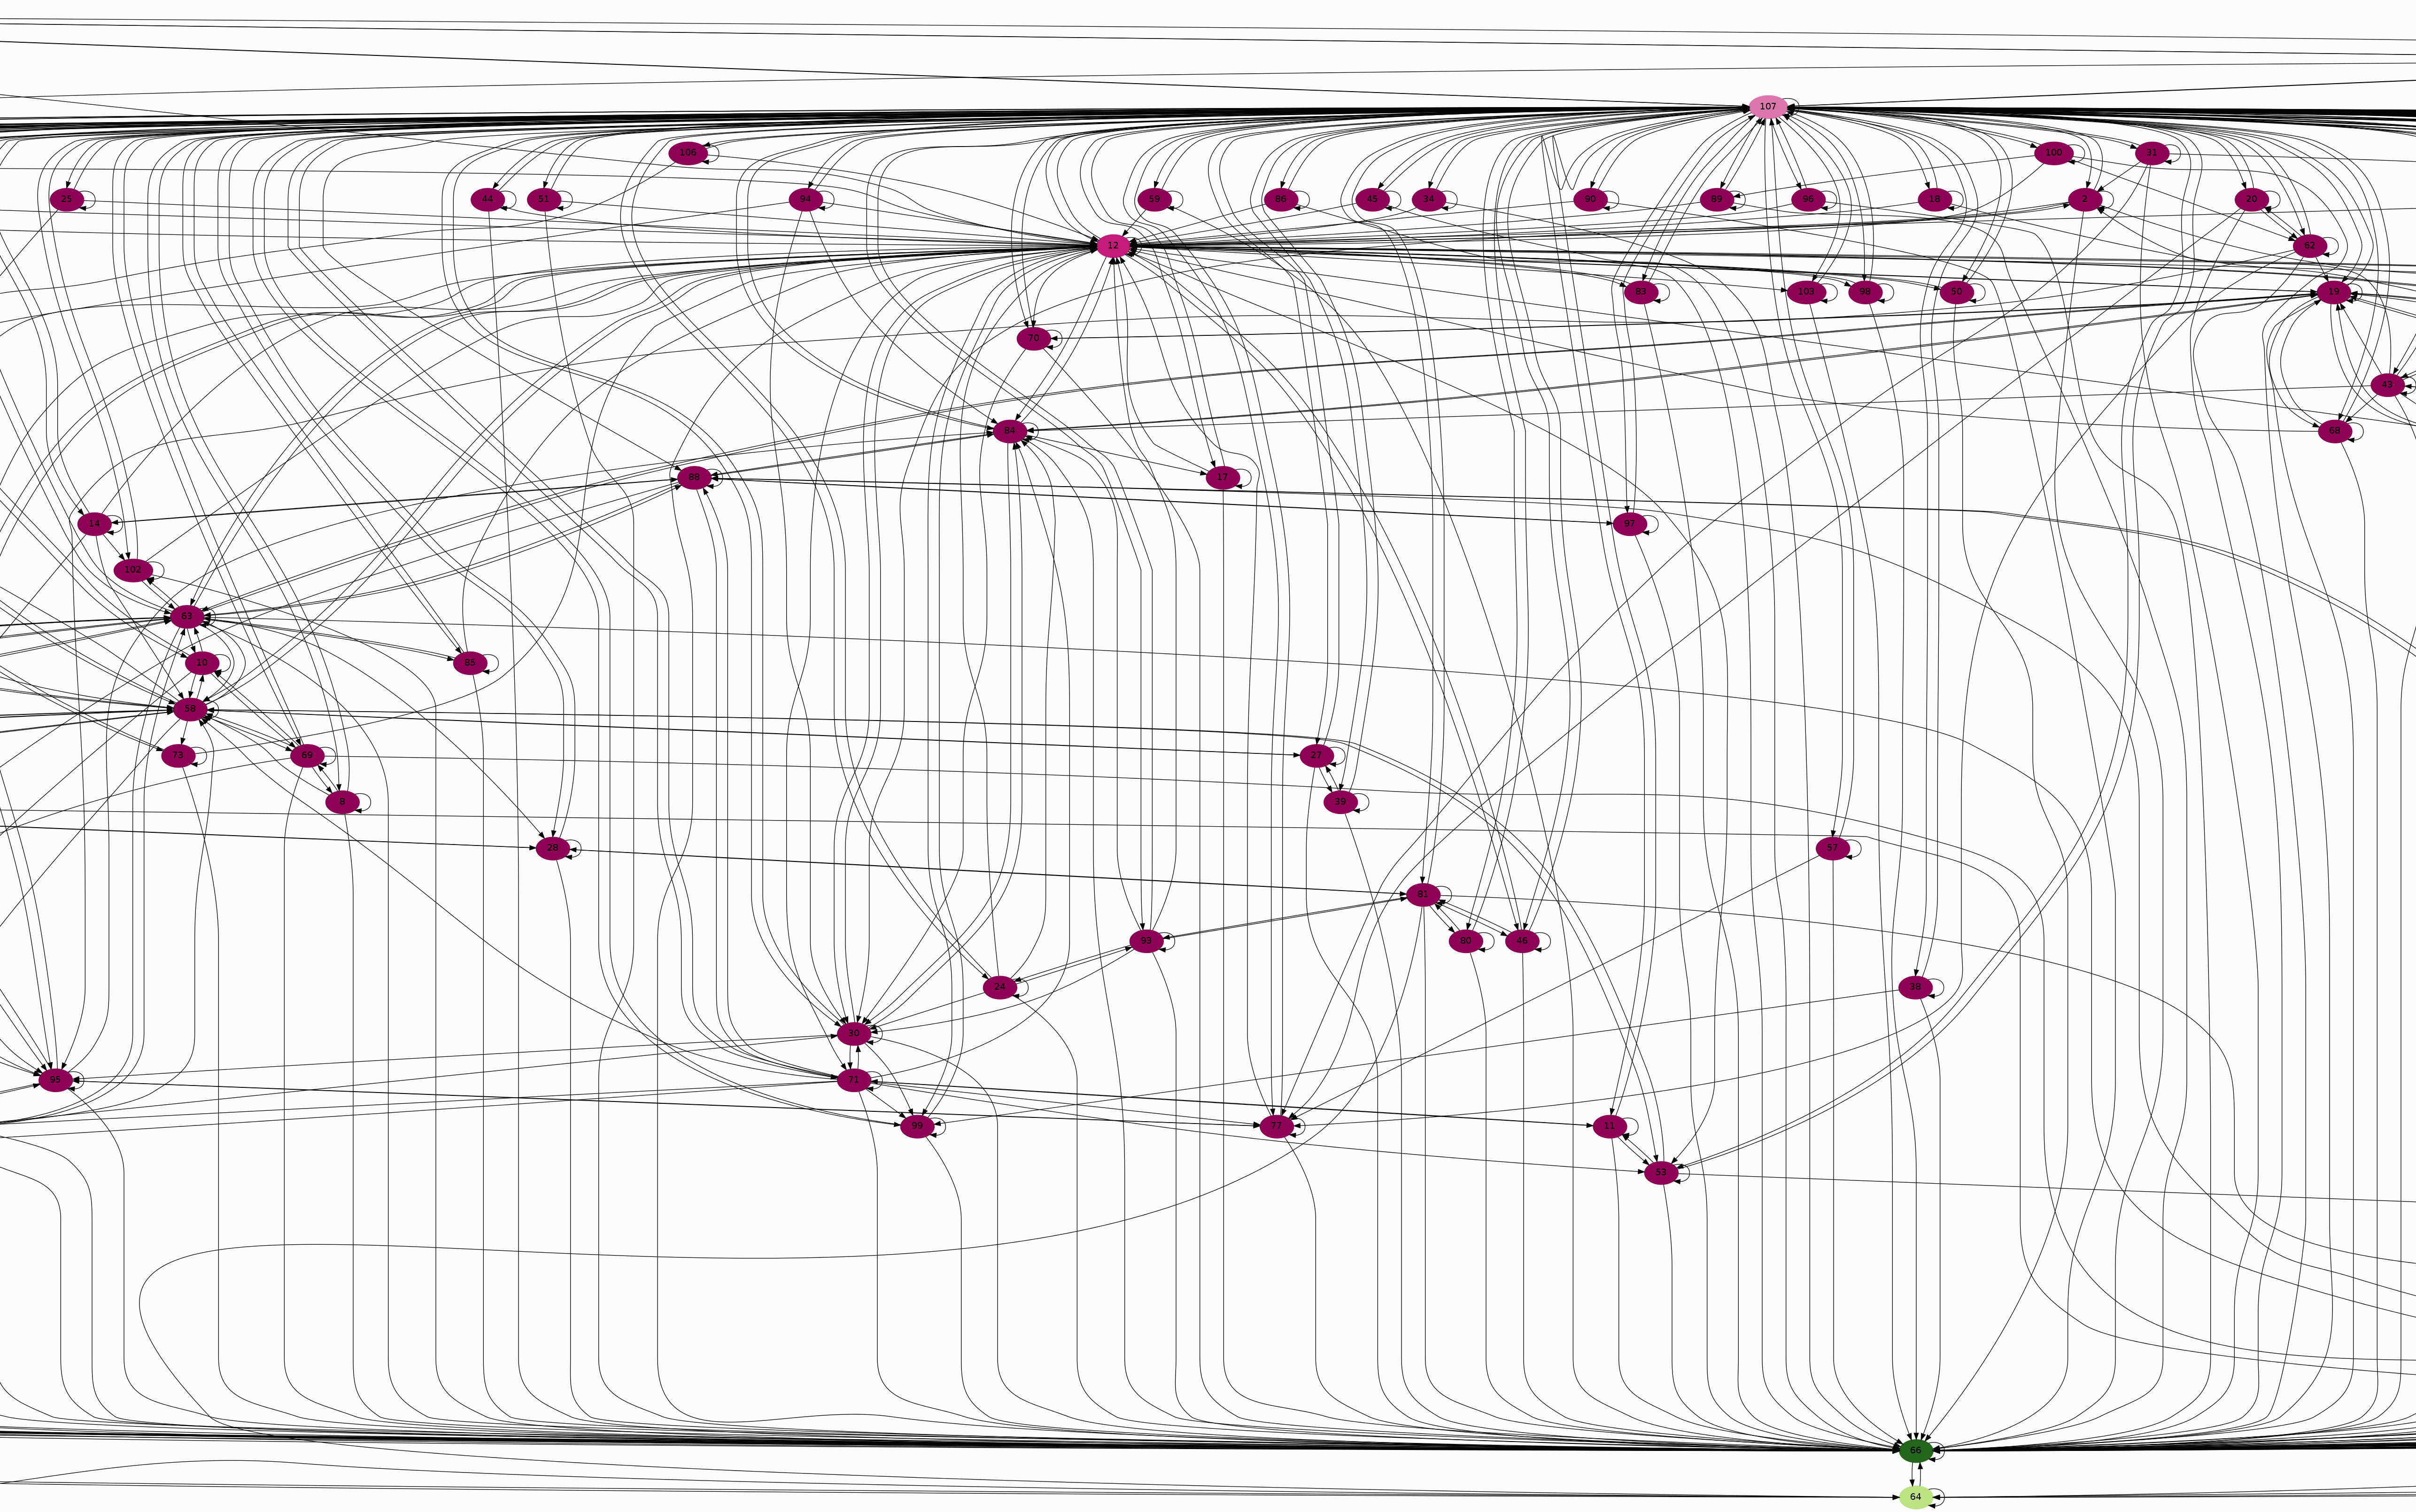
\includegraphics[height=1\textheight]{graphics/pr_overview.png}
  \caption[labelInTOC]{}
  \label{fig:prOverview} 
\end{center}
\end{figure}
\end{frame}

\begin{frame}[c]
    \myframetitle{Page-Rank}{PR ist hoch bei hohem In-Degree}
    %\usepackage{graphics} is needed for \includegraphics
\begin{figure}[htp]
\begin{center}
  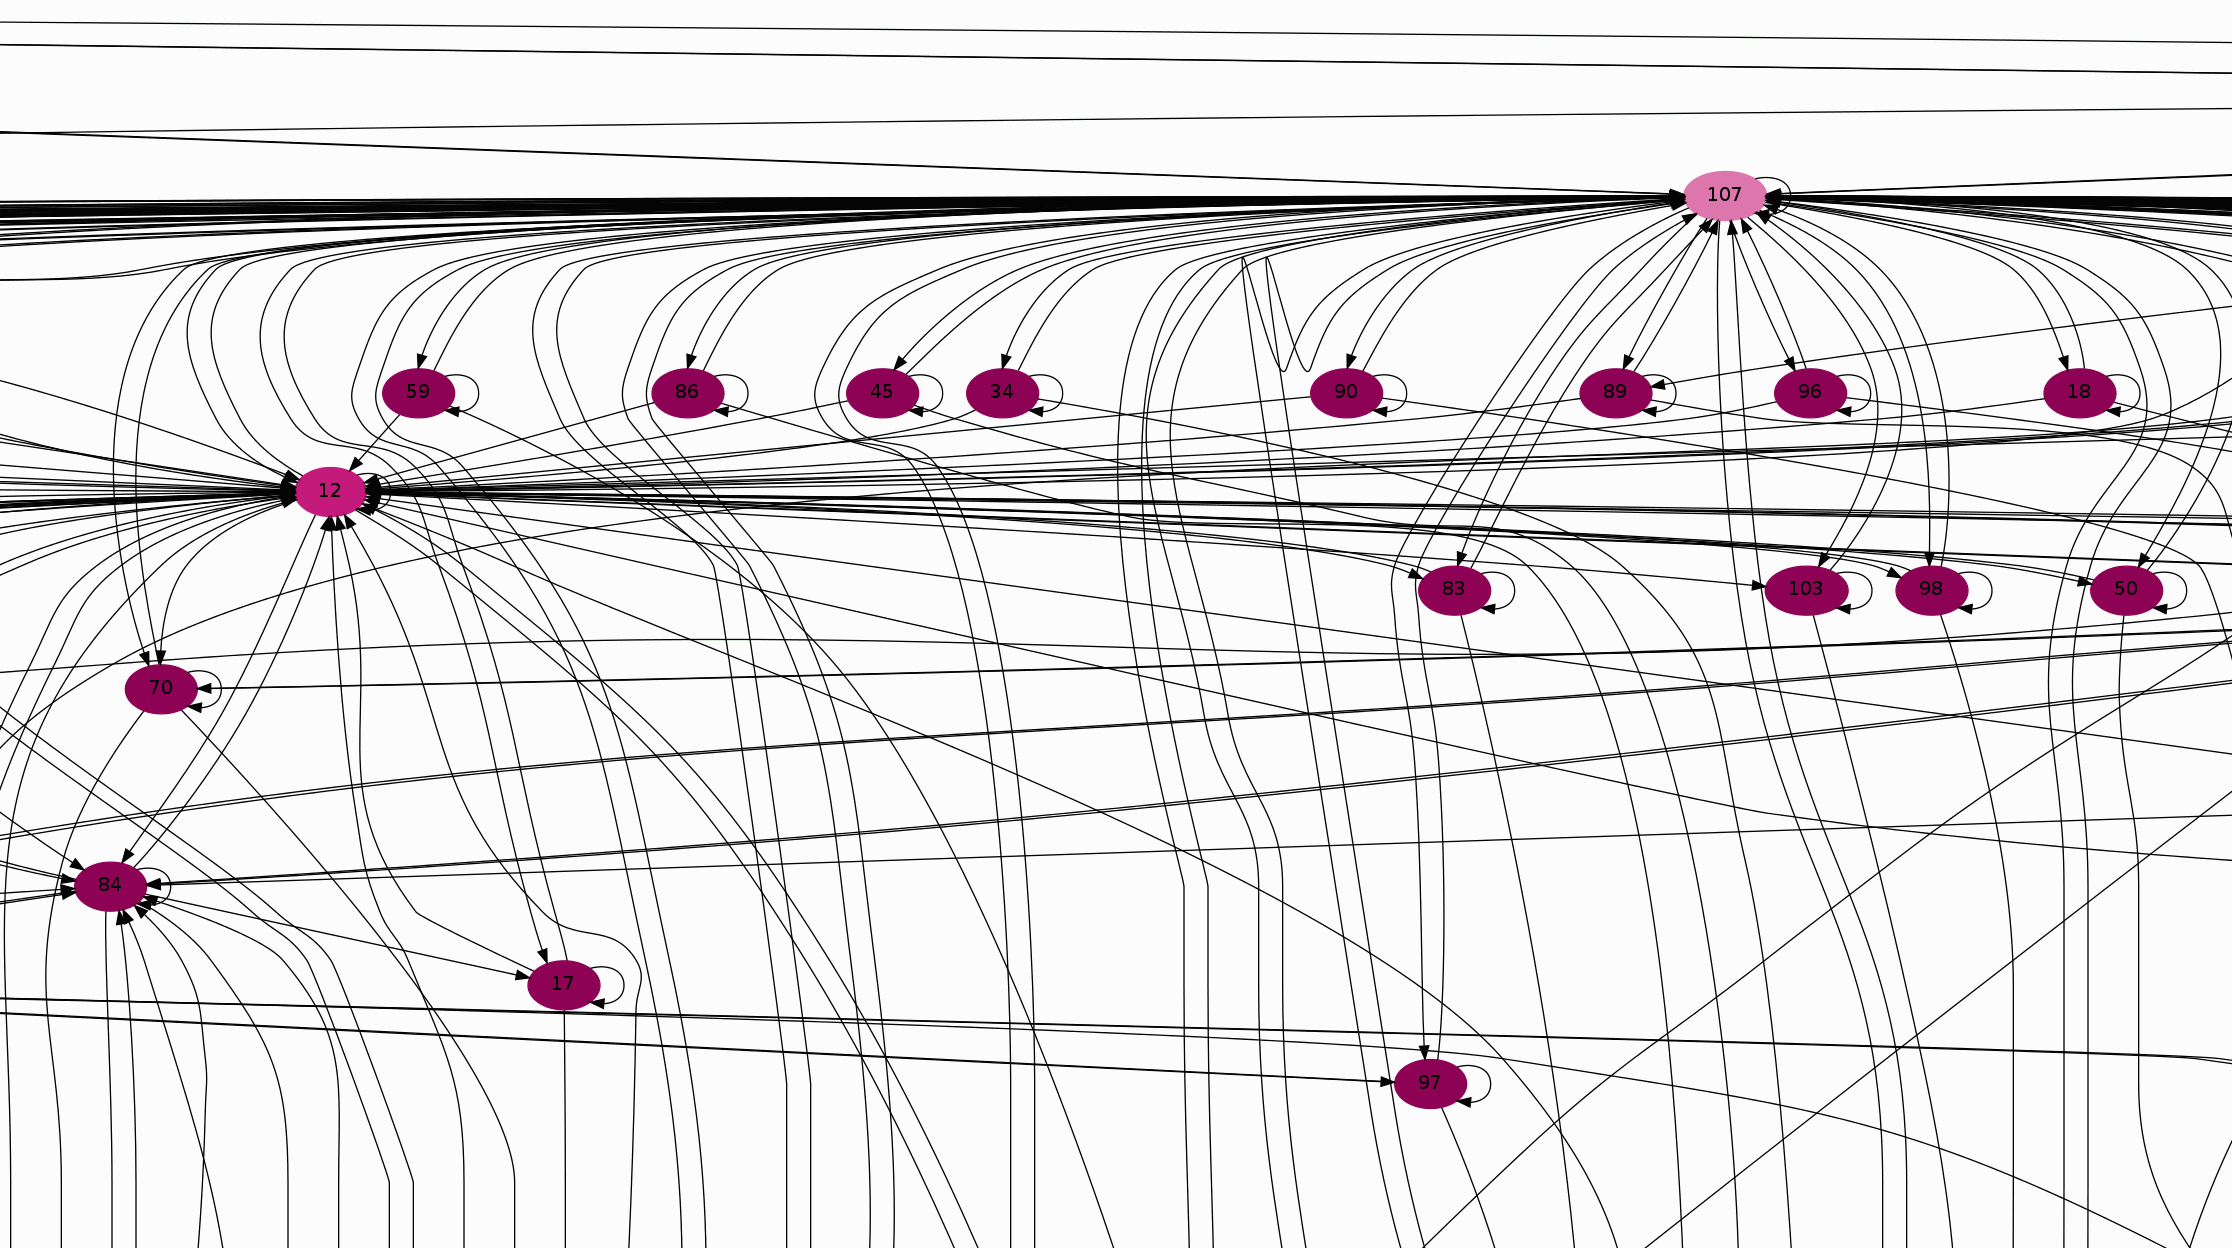
\includegraphics[height=1\textheight]{graphics/pr_high_inout_degree.png}
%  \caption[labelInTOC]{}
%  \label{fig:hihg_inoutdegree}
\end{center}
\end{figure}

\end{frame}


\begin{frame}[c]
    \myframetitle{Page-Rank}{PR ist hoch bei kleinem Out-Degree der Vorgänger}
%\usepackage{graphics} is needed for \includegraphics
\begin{figure}[htp]
\begin{center}
  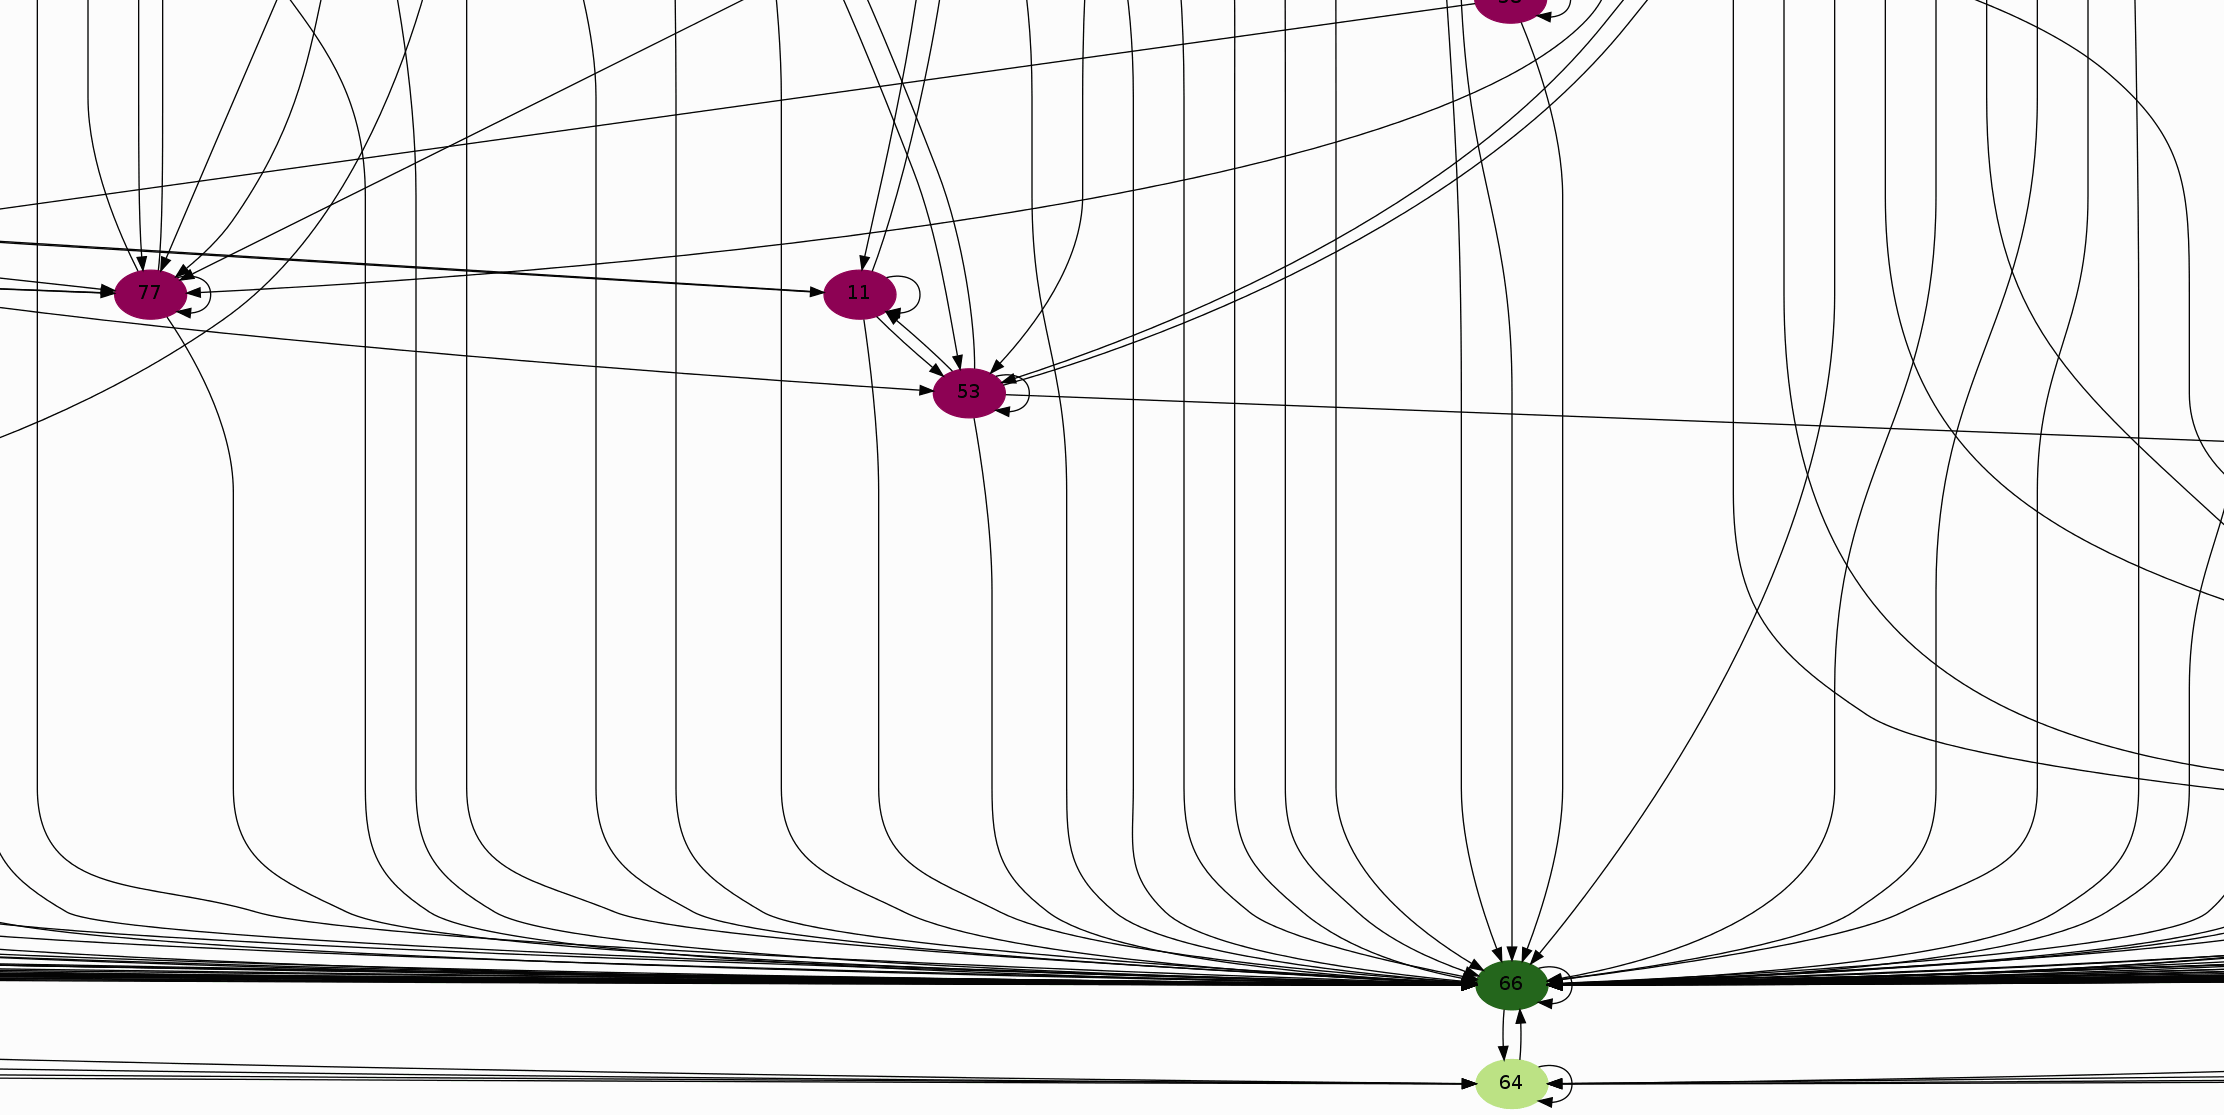
\includegraphics[height=1\textheight]{graphics/high_indegree.png}
%  \caption[labelInTOC]{}
%  \label{fig:prHighIndegree}
\end{center}
\end{figure}
\end{frame}

\begin{frame}[c]
    \myframetitle{Page-Rank}{Ranking des Graphen aus Aufgabe 1}
    \begin{itemize}
  \fatitem{Für den Graph aus Aufgabe 1 ergibt sich folgendes Ranking:}
\begin{enumerate}
  \item ID(66)	PR(0,28804), Special Categories
  \item ID(64)	PR(0,22126), Wikipedia Categorization
  \item ID(107) PR(0,06453), Category Data mining
  \item ID(12)	PR(0,03134), Data mining
  \item ID(91)	PR(0,01396), Why  might a category list\ldots
  \item ID(58)	PR(0,01061), Cluster analysis
\end{enumerate}
\ldots
\begin{enumerate}[100.]
\item  ID(104)	PR(0,00223), Affinity analysis
\end{enumerate}
\item Max(PR)=0,28804 Min(PR)=0.00223
\item Die Wahrscheinlichkeit durch zufälliges Surfen auf die Seite
``Special Categories'' zu kommen beträgt demnach 28\%
\item Die Wahrscheinlichkeit durch zufälliges Surfen auf ``Affinity Analysis'' zu
kommen beträgt nur 0.2\%
\end{itemize}
\end{frame}
